\documentclass[a4paper,english,french]{article}
\usepackage{source/packages/preamble}

\setlength\parskip{1em plus 0.1em minus 0.2em}
\declaretheorem[thmbox=S,style=definition]{theorem}

\begin{document}

This document is an example showing the different functionalities of this boilerplate. It can also be used as a quick cheat sheet to find how to write quickly things.

\begin{figure}
    \centering
    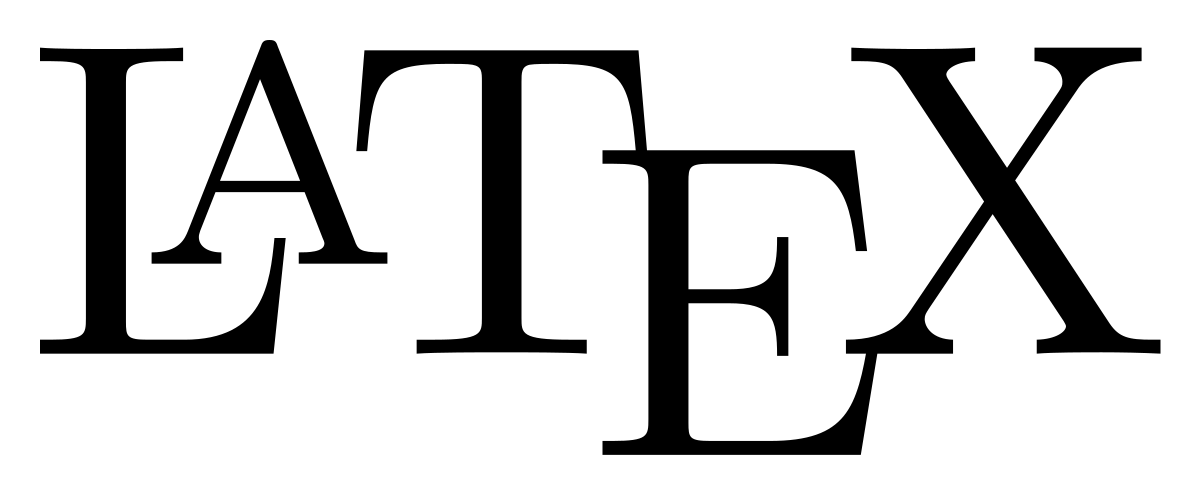
\includegraphics[width=3cm]{LaTeX}
    \caption{An example of image integration}
\end{figure}

Notice that we do not have to specify the path of the image. By default, the image will be searched in \texttt{source/images/}. Also, \texttt{UseLATEX.cmake} allows to insert almost any image format: it will be converted internally before being inserted in the document. That's why the image extension doesn't need to be included.

\subfile{source/partials/sample}

\end{document}
